\chapter{Lecture 17 - Extended Surfaces Heat Exchanger}
\label{ch:ch17}
\section{Objectives}
The objectives of this lecture are:
\begin{enumerate}
\item Discuss motivation for heat exchangers with extended surfaces.
\item Describe a correlation for estimating the friction factor for such a heat exchanger
\end{enumerate}

\section{Extended Surfaces Heat Exchangers}
\newthought{In previous lectures} we have discussed a range of different heat exchangers for energy conversion applications.  

\begin{itemize}
\item For PWRs a recirculating u-tube steam generator provides heat transfer from the subcooled liquid water of the primary to a low-quality saturated mixture of the secondary.  Heat transfer performance on both the primary and secondary side of the heat exchanger is excellent.

\begin{marginfigure}
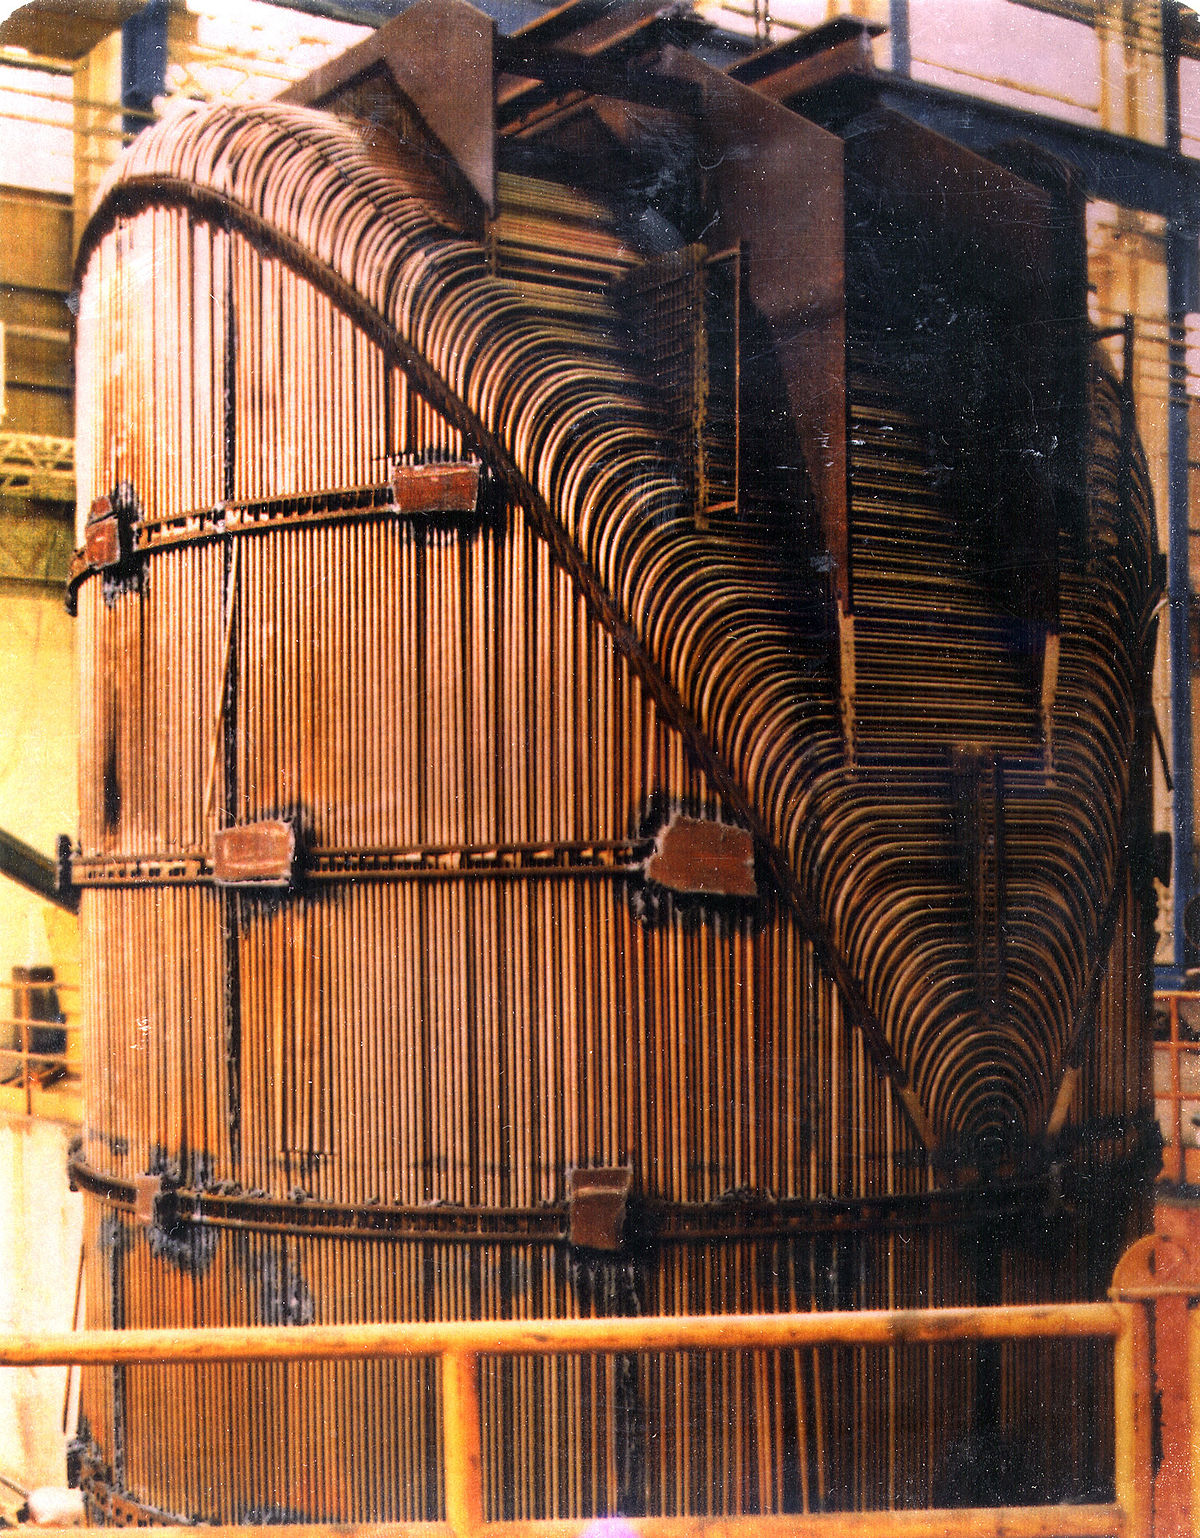
\includegraphics{SG.png}
\caption{Steam generator internals.}
\label{fig:SG}
\end{marginfigure}

\item The condenser of Rankine cycles provides heat transfer between the high-quality saturated mixture of turbine exhaust and subcooled liquid of the condenser cooling water.  Closed feedwater heaters in Rankine power conversion cycles work with similar fluids.

\item A reheater employed in a Rankine cycle is used to transfer heat from a saturated steam to a lower-temperature and pressure saturated steam.  

\begin{marginfigure}
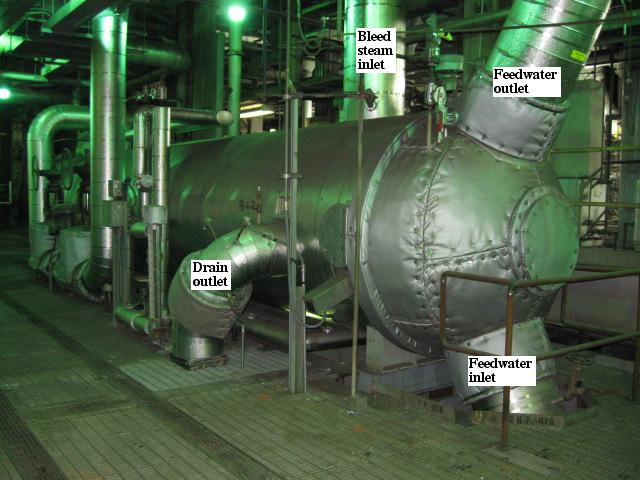
\includegraphics{CFWH.png}
\caption{Closed feedwater heater.}
\label{fig:CFWH}
\end{marginfigure}

\item An inter-cooler or precooler used in a Brayton power cycle rejects heat from a gas working fluid to some cooling medium.  

\item A regenerator used in a Brayton cycle has gas on both the high- and low-temperature side of the heat exchanger.  
\end{itemize}

What we have not done is investigate in any level of detail the thermal or hydraulic performance of these devices; we simply drew them as boxes on our schematics and assumed that they would function as specified. For some applications, especially those for which at least one side of the heat exchanger is a gas, special measures are called for to enhance convective heat transfer performance.  One such measure is the use of ``extended surfaces.''  

\newthought{An early application} of extended surfaces for enhanced heat transfer was with the MAGNOX reactor.\sidenote{MAGNOX = ``magnesium non-oxidizing.''} This reactor comprised natural uranium fuel, graphite moderator and carbon dioxide as the coolant.  In order to enhance convective heat transfer to the gas coolant, spiral ribs and fins were incorporated into the clad structure as illustrated in Figure \ref{fig:magnox}.

\begin{marginfigure}
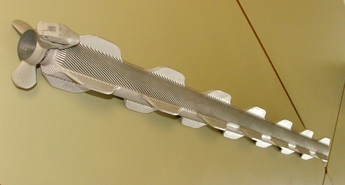
\includegraphics{magnox.png}
\caption{Magnox fuel can.}
\label{fig:magnox}
\end{marginfigure}

Heat exchangers with extended surfaces are envisioned for use in Gen IV reactor concepts in which heat transfer occurs between highly conductive fluids---such as liquid lead or sodium---and fluids that conduct heat poorly such as carbon dioxide, air, or helium.\marginnote{\textbf{Nusselt number} is a non-dimensional parameter that characterizes the convective heat transfer capability of a fluid relative to thermal conductivity.  
\index{Nusselt number}

$$\text{Nu} = \frac{hL}{k}$$
where $h$ is the convective heat transfer coefficient, $k$ is the thermal conductivity and $L$ is some characteristic length, such as a pipe diameter.} The idea is to disrupt the thermal boundary layer on the side where heat transfer would otherwise be poor by using surface features that force complex flow behavior near the heat transfer surface.  The benefit is improved convective heat transfer; the price we pay is increased hydraulic pressure losses.  

A desirable extended surface design is one where the convective enhancement outweighs the hydraulic penalty. If we wanted to quantify this trade-off, a thermal performance factor,\cite{maradiya2018heat} such as $\eta$ shown in Equation \ref{eq:tpf} might be defined.
\index{thermal performance factor}
\begin{equation}
\eta = \frac{\sfrac{\text{Nu}}{\text{Nu}_0}}{(\sfrac{f}{f_0})^{1/3}}
\label{eq:tpf}
\end{equation}
Sadly, this sort of an analysis is beyond the scope of this course.


\newthought{In this lecture} we will describe hydraulic correlations for two extended surface concepts:  

\index{extended surface heat exchanger}
\begin{itemize}
\item Helical rib or fin; and
\item twisted tape insert
\end{itemize} 
\index{Fanning friction factor}
Both correlations provide a way to calculate a Fanning friction factor, $f^{\prime}$,\marginnote{\textbf{Fanning friction factor}, $f^{\prime}$ is related to the Darcy friction factor, $f$, by a factor of 4} from which we can calculate hydraulic pressure losses for flow along a specified length $(L)$ of enhanced pipe of a given diameter $(D)$ using the equation below:
$$\Delta p = 4 f^{\prime} \left(\frac{L}{D} \right)\rho \left(\frac{v^2}{2} \right)$$
\textbf{Important note:} when using USCS units, the equation for pressure drop must be modified to include $g_c$:
$$\Delta p = 4 f^{\prime} \left(\frac{L}{D} \right)\rho \left(\frac{v^2}{2g_c} \right)$$
where $\rho$ is given in lb$_{\text{m}}$/ft$^{3}$ and $p$ is in lb$_{\text{f}}$/ft$^{2}$ and $g_c = 32.2$ lb$_{\text{m}}$/lb$_{\text{f}}$ ft/s$^{2}$. \marginnote{Students are strongly encouraged to work through the units of these equations for $\Delta p$ to make sure it is clear why $g_c$ is needed in USCS units.}

In a homework exercise later in the course we will describe similar corrrelations for Nusselt number to allow us to estimate changes in thermal performance.

\section{Helical Rib or Fin}
This correlation is for circular tubes enhanced with helical ribs or fins.  The correlation\cite{ravigururajan1999comparative} we will use estimates the Fanning friction factor relative to the friction factor of a smooth tube as a function of the following parameters:
\begin{itemize}
\item Reynolds number $(\text{Re})$.
$$29.1\text{Re}^{Y1}$$
$$Y1 = 0.67-0.06\frac{p}{D}-0.49\frac{\alpha}{90}$$ 
where $p$ is the rib separation distance, $\alpha$ is the helix angle measured in degrees, and $D$ is the maximum tube inside diameter. 
\item Rib height $(\epsilon)$.
$$\left(\frac{\epsilon}{D} \right)^{Y2}$$
$$Y2 = 1.37 - 0.157 \frac{p}{D}$$
\item Rib pitch $(p)$---distance of rib separation:
$$\left(\frac{p}{D} \right)^{Y3}$$
$$Y3 = -1.66\times10^{-6}\text{Re}-0.33\frac{\alpha}{90}$$
\item Helix angle $(\alpha)$
$$\left(\frac{\alpha}{90} \right)^{Y4}$$
$$Y4 = 4.59+4.11\times10^{-6}\text{Re}-0.15\frac{p}{D}$$
\item Contact angle $(\beta)$ and number $(n)$ of sharp corners 
$$\left(1+\frac{2.94}{n} \right)\sin{\beta}$$
\begin{marginfigure}
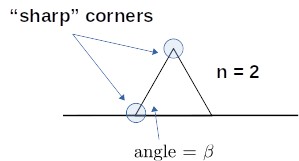
\includegraphics{contact_angle.png}
\caption{Contact angle and sharp corners for a rib.}
\label{fig:contact_angle}
\end{marginfigure}
where $\beta$ and $n$ are as shown in Figure \ref{fig:contact_angle}.

\end{itemize}
The reference smooth-tube friction factor is given as:
$$f^{\prime}_{\text{sm}}=\left(1.58\ln{(\text{Re})}-3.28 \right)^{-2}$$
and the complete correlation is formed in Equation \ref{eq:R-B}.

\begin{equation}
\frac{f^{\prime}_a}{f^{\prime}_{\text{sm}}} = \left\{1+\left[29.1\text{Re}^{Y1}\left(\frac{e}{D} \right)^{Y2}\left(\frac{p}{D}\right)^{Y3}\left( \frac{\alpha}{90}  \right)^{Y4} \left(1+\frac{2.94}{n} \right) \sin{\beta} \right]^{\sfrac{15}{16}} \right\}^{\sfrac{16}{15}}
\label{eq:R-B}
\end{equation}

Quoting from the course textbook, ``...this correlation predicts 96\% of the database to within 50\% and 77\% [of the database] to within 20\%.'' from which you should understand that high precision should not be expected.

\section{Twisted Tape Insert} \index{twisted tape correlation}
\newthought{Twisted Tape inserts} are a widely used class of swirl-flow inducing devices.  Their advantages over helical ribs include:
\begin{itemize}
\item relative ease of manufacture and installation;
\item allows for retrofitting by swapping out inserts
\end{itemize}
The course textbook provides multiple correlations for laminar and turbulent flow.  In these notes I will briefly present only the turbulent flow correlation.\cite{manglik1993heat}

This friction factor is presented as a function of:

\begin{itemize}
\item Reynolds number
\item Tape thickness $(\delta)$
\item Tape half-pitch $(H)$\marginnote{\textbf{tape half-pitch} is the axial length for the tape to take a 180 degree twist.}
\item ``Twist Ratio'' $(y)$ which is just the half-pitch divided by the pipe diameter:
$$y = \frac{H}{D}$$
\end{itemize}

The friction factor correlation is given by Equation \ref{eq:twisted-tape}.

\begin{equation}
f^{\prime}=\frac{0.0791}{\text{Re}^{0.25}}\left[1+\frac{2.752}{y^{1.29}} \right]\left[\frac{\pi}{\pi - \left(\sfrac{4 \delta}{D} \right)} \right]^{1.75} \left[\frac{\pi +2 - \left(\sfrac{2\delta}{D} \right)}{\pi - \left(\sfrac{4 \delta}{D} \right)} \right]^{1.25}
\label{eq:twisted-tape}
\end{equation}
where $f^{\prime}$ is again the Fanning friction factor for the following range of conditions:
$$ \text{Re} \ge 10^4, \ \ 2 \le y \le \infty, \ \ 0.03 \le \sfrac{\delta}{D} \le 0.83$$

\section{Summary}
In this lecture we discussed two correlations for hydraulic pressure drop for tubes with convective heat transfer enhancements.  We did not discuss the actual convective enhancements, we only discussed the correlation to predict the attendant hydraulic pressure losses.  The corresponding correlations for convective heat transfer will be treated in a set of homework problems.
